\documentclass[border=10pt]{standalone}
\usepackage{tikz}
\usetikzlibrary{shapes}

\begin{document}
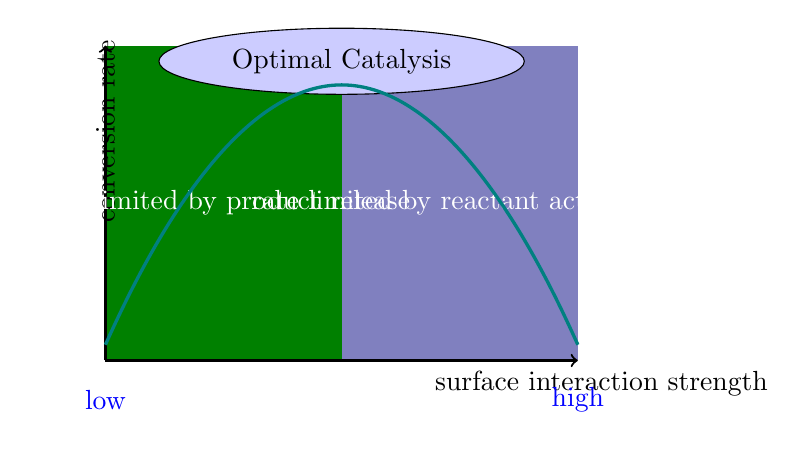
\begin{tikzpicture}
    % Background regions
    \fill[green!50!black] (0,0) rectangle (3,4);
    \fill[blue!50!black!50] (3,0) rectangle (6,4);
    
    % Axes
    \draw[->, thick] (0,0) -- (0,4) node[left, rotate=90, pos=1.05] {conversion rate};
    \draw[->, thick] (0,0) -- (6,0) node[below, pos=1.05] {surface interaction strength};
    
    % Axis labels
    \node[blue] at (0,-0.5) {low};
    \node[blue] at (6,-0.5) {high};
    
    % Region text
    \node[text=white] at (1.5, 2) {rate limited by product release};
    \node[text=white] at (4.5, 2) {rate limited by reactant activation};
    
    % Optimal Catalysis ellipse
    \node[ellipse, draw, fill=blue!20, text width=3cm, align=center, inner sep=4pt] at (3,3.8) {Optimal Catalysis};
    
    % Conversion rate curve
    \draw[teal, very thick] (0,0.2) parabola bend (3,3.5) (6,0.2);
    
\end{tikzpicture}
\end{document}